\begin{figure}[t]
\centering
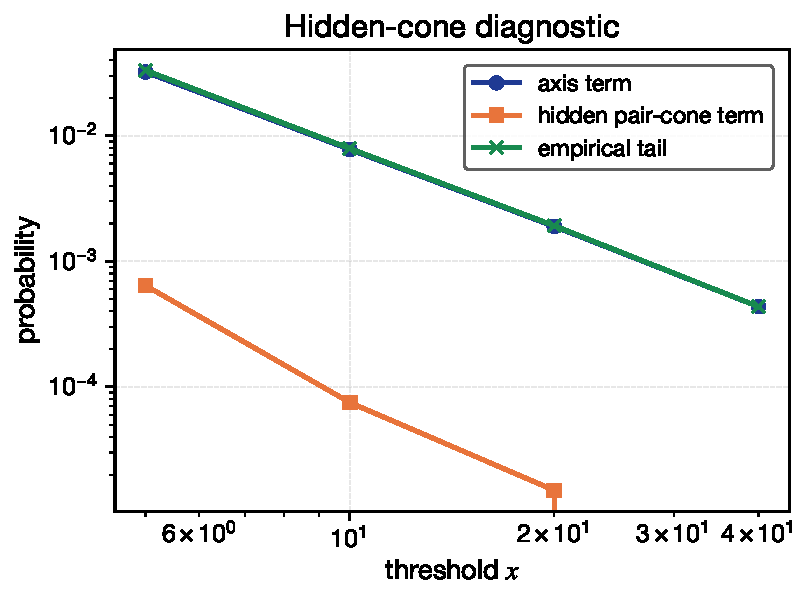
\includegraphics[width=0.85\linewidth]{figures/F13_hidden_cones_placeholder.pdf}
\caption[Hidden-cone diagnostic]{Axis exceedance term (blue), hidden pair-cone term (orange), and empirical sum-tail (green). The hidden-cone scale $\overline H_2(x) \propto x^{-\alpha_2}$ with $\alpha_2 = 3$ decays faster than the axis scale $\alpha = 2$, so the hidden term sits below the axis term at every threshold; the gap is the hidden-cone mass quantified by Theorem~\ref{thm:hidden-second-order}.}
\label{fig:hidden-cones-placeholder}
\end{figure}
